\section{Lippukunnanjohtajan tervehdys}

\begin{multicols}{2}
\noindent Jälleen yksi toiminnantäyteinen partiovuosi on vierähtänyt ja 
pian on aika rauhoittavan joululoman ennen seuraavan vuoden partioseikkailuja. Myös 
edellisestä Tassusta on ehtinyt vierähtää jo useampi vuosi. Erityiskiitos 
uuden päätoimittajan rusakoiden oma lippukuntalehti on saanut tuulta 
purjeisiinsa ja me kaikki pystymme palaamaan kuluneen vuoden tapahtumiin 
erilaisten juttujen ja kuvien merkeissä -- jo 75. kertaa!

Ehkä ensimmäistä kertaa koskaan Tassusta löytyy ei yksi, ei kaksi, vaan 
peräti kolme raporttia vuoden aikana suoritetuista nahkaliljavaelluksista 
(s.~\pageref{section:vihreaNahkalilja}, \pageref{section:mustaNahkalilja} ja 
\pageref{section:punainenNahkalilja}). Nahkaliljat ovat partiomerkkejä, joiden 
tarkoituksena on korostaa ulkoilun merkitystä ja motivoida partiolaisia 
ylläpitämään ja kehittämään peruskuntoaan. Ruumiillisesti ja henkisesti 
kuormittavat vaellukset ovat vartiossa toimimista parhaimmillaan, tapahtuvat 
luonnossa ja muuttuvat nousujohteisesti yhä haastavammiksi taitettavan matkan 
pidentyessä; juuri päivitetyssä partiomenetelmässä käytetään ilmaisuja 
ryhmässä toimiminen, toiminta luonnossa ja oma partiopolku -- voihan 
vaelluksia kutsua myös elämyksiksi.

Ei uutta ilman vanhaa, myös partioliikkeen perustaja Baden"-Powell painottaa
terveyden ja liikunnan tärkeyttä viimeisessä viestissään partiolaisille: 
''Ensi askel onneen on tämä: kasvata itsesi terveeksi ja voimakkaaksi, niin 
että vartuttuasi voit olla hyödyksi ja siten nauttia elämästä.'' 
Terveyteen kuuluu muitakin ulottuvuuksia kuin fyysinen terveys ja partion 
tavoitteena on kasvattaa lapsista ja nuorista persoonallisuudeltaan ja 
elämäntavoiltaan tasapainoisia yhteiskunnan jäseniä.

Partiomenetelmää sovelletaan kaikkeen toimintaan partiossa: viikkokokouksiin, 
erilaisiin retkiin, paraateihin, kilpailuihin, leireihin, vaelluksiin, juhliin 
ja muihin tapahtumiin. Tassu voi olla paljon muutakin kuin sanallista ja 
kuvallista kuvausta toiminnasta. On tärkeää, että lippukuntalehti on 
lippukuntansa näköinen. Mikäli haluaisit osallistua lehden tekemiseen, vedä 
rohkeasti päätoimittajan hihasta. Osallistu ainakin Tassun kuvakilpailuun. 
Löydät ohjeet sivulta~\pageref{section:kuvakilpailu}!

Partioterveisin

Janne

\medskip

\noindent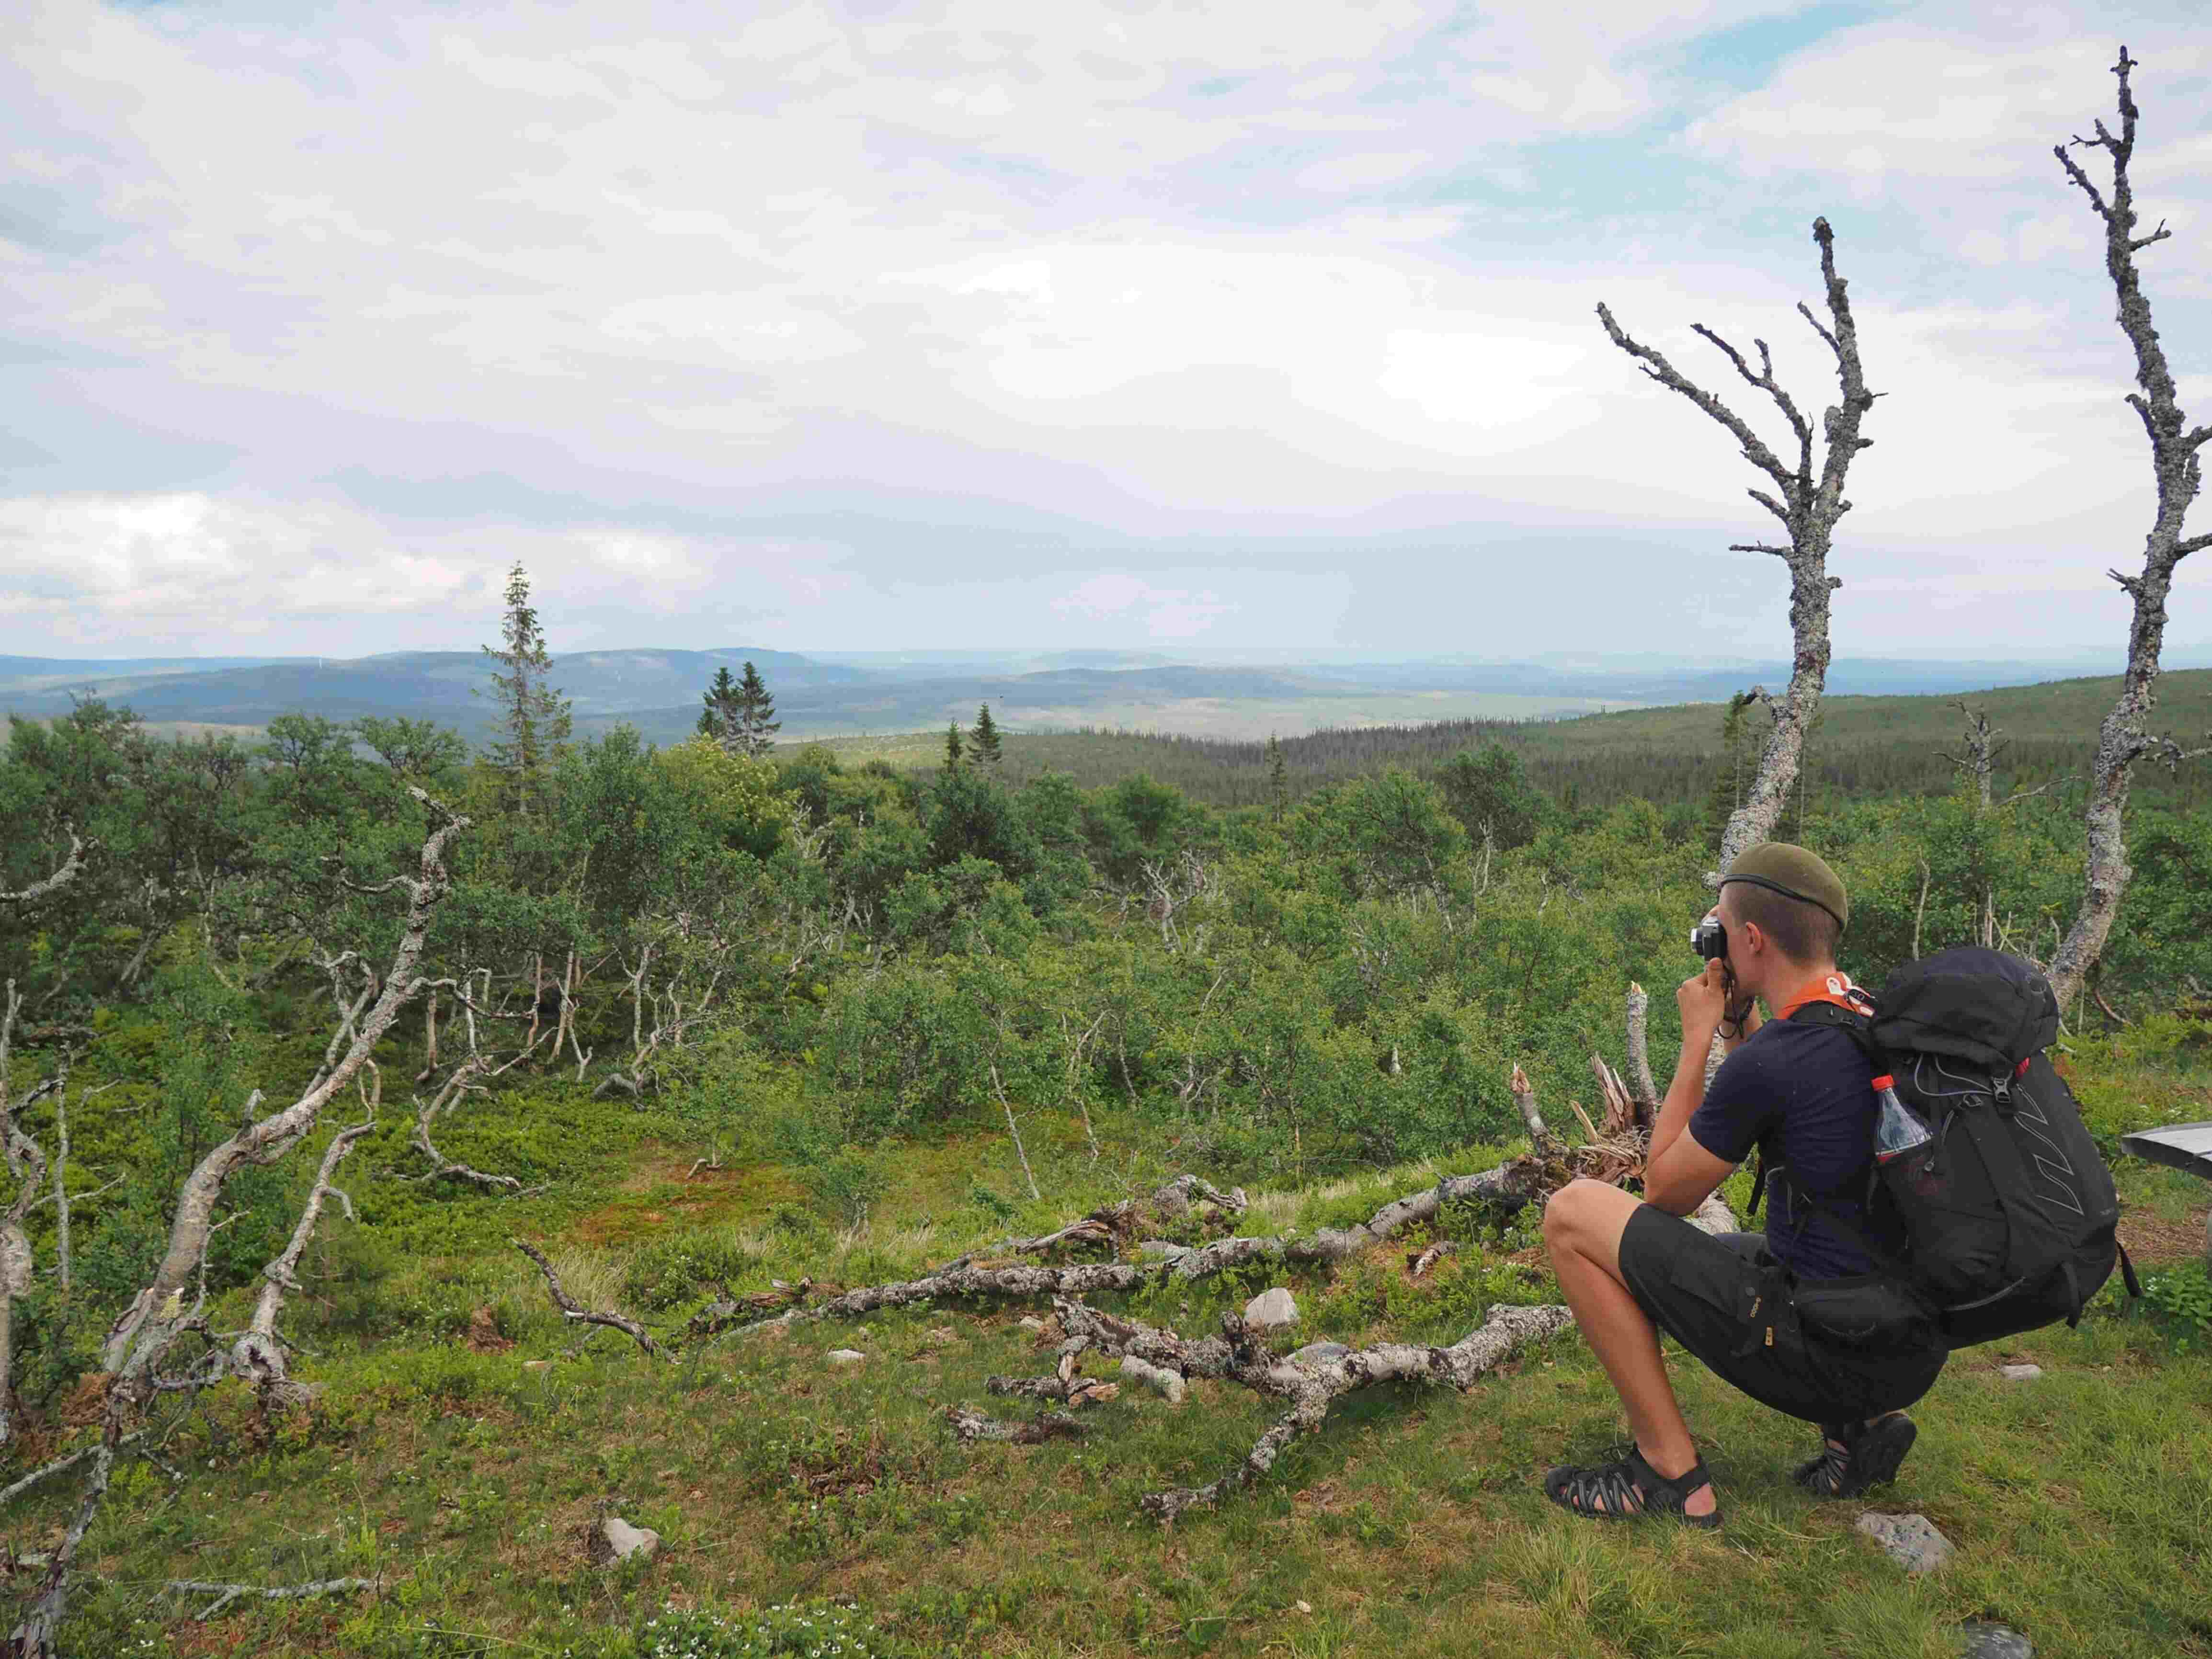
\includegraphics[width=\linewidth,trim={0 1.5cm 0 4cm},clip]{assets/lpkjtervehdys}

\medskip

\noindent\null\hfill Kuva: Tanguy Gérôme
\end{multicols}
